\documentclass{proc}
\usepackage{hyperref}
\usepackage{graphicx}

\begin{document}

\title{One day of SHMetro}

\author{Yuting Han, Meijie Wang}

\maketitle

\section{Introduction}
One of the main characteristics of cities is high-frequency people streaming. These flows are reflected in all the subways dashing through the city. With our visualizations, we want to give an impression of this pulse of the city from the perspective of Shanghai Metro Visualization. In this project, we collect Shanghai’s metro datasets in 2015/04/20. Our data are collected from Shanghai public transportation released by Shanghai government in 2015 (http://soda.shdataic.org.cn).  

We mainly focus on metro streaming and passenger streaming in different stations along the timeline on a particular day. From the results of our project, people can easily observe the metro schedule and passenger volume details horizontally and vertically. To be specific, we visualize the real-time traffic flow and detailed passenger flow interactively and present how metro trains and passenger volume are distributed along time within one day.


\section{Related Work}
User-centered design ideology and method is proposed by a group of researchers in 2016. They identify general design requirements for visualizing uncertainty on mobile applications as well as domain-specific design requirements for visualizing uncertainty in transit arrival times \cite{1}. 

In IEEE VIS 2014 Arts Program, researchers presented an artistic visualization exhibit providing three plus one perspectives into the complex system of a metropolitan subway network. Each visualization combines established techniques with a highly aesthetic form in order to attract people to observe and dwell on different aspects of urban mobility  \cite{2}.

In 2015, researchers introduced the basic concept and pipeline of traffic data visualization, provides an overview of related data processing techniques, and summarizes existing methods for depicting the temporal, spatial, numerical, and categorical properties of traffic data \cite{3}. 

The techniques they mentioned is worth learning. In 2013, researchers published Visual Traffic Jam Analysis Based on Trajectory Data, they presented an interactive visual analysis system to analyze traffic jams on a large scale road network in real life. They build a visual interface for interactive exploration of the detected traffic jam information both in detail on a road segment as well as on a higher level in a spatial view on a map and in a small multiples view with propagation graphs \cite{4}. 

In 2013 IEEE 14th International Conference on Mobile Data Management, researchers from The Hong Kong University of Science and Technology presented an interactive visual analytics system, T-Watcher, for monitoring and analyzing complex traffic situations in big cities via taxi trajectory data \cite{5}. Researchers from MIT Senseable City Laboratory has published a paper about a visualization technique to highlight the impact that traffic incidents have on congestion. They draw attention to a road incident through the use of an expanding circle that reveals the state of the road network in the immediate vicinity of the incident, thereby enabling users to see the before and after effects of the incident \cite{6}. Researchers from MIT Senseable City Laboratory also published a paper introduce Touching Transport, a case study enabling casual exploration of urban mobility in Singapore through a set of visualizations on a multi-touch tabletop \cite{7}. Till Nagel from MIT Senseable City Lab also published a paper presenting a tabletop visualization of relations between geo-positioned locations \cite{8}.  

\section{Methods}
\subsection{Data cleaning method}
Raw data is messy and data cleaning work counts for 70 percentage workload. To integrate data for metro flow visualization, both time and spatial data are required. And to convey the info of how metro flow frequency affected by time, line number and section of a line, all such data is needed to be compact into one JSON file.

\subsection{Visualization method}
Three pages are designed for metro data visualizations, traffic flow, entrance flow, and exit flow. And for technical tools, we use D3.js and Jquery.js library for our projects mainly. Especially, Scroll CSS method is used to control the pinned part and the rolling part in the web page. In the “Entrance Flow” and the “Exit Flow” pages, we design the metro map set in a fixed position while the heat map on the right rolling as the mouse slides. Scroll solved this problem. For the visualization, we design several interactive visualization graphs to present multiple dimensions of information.
\subsubsection{Traffic Flow}
The interactive graph in Traffic Flow page presents a real-time metro map where the train is located. Each highlighted moving point is one metro train and it moves along the metro line. Users can have an overall intuition of the metro flow in Shanghai. For example, dense moving points deliver that now it is rush hour, while sparse moving points convey that the traffic is not busy. 

Two interactive views are designed. First, the button on the right can be clicked to control which metro line to be presented in the graph. The click of the metro line button can make the line highlighted. Second, the timeline on the bottom are designed to select time periods to be presented. From these interactions, details of how metro trains move as time goes become clear. 

\begin{figure}[t]
	\centering
	\includegraphics[width=0.5\textwidth]{img/TrafficFlow}
	\caption{TrafficFlow}
	\label{fig:curve}
\end{figure}

\subsubsection{Entrance Flow}
The Entrance Flow page visualized passenger volume information versus metro station. The data displayed are the amount of passenger who enters the metro station. 

There are two main parts of this page. The first half of Entrance Flow page presents information about all metro stations in Shanghai. Photos of metro stations stand in rows and are sorted by line. When the user clicks a photo of one metro station, the detailed information of that metro station will be shown below the photo gallery. The detailed information includes a zoomed out photo of the metro station, the geographic information and a highlighted point shown in the Shanghai metro map, which is useful for urban researchers.

\begin{figure}[t]
	\centering
	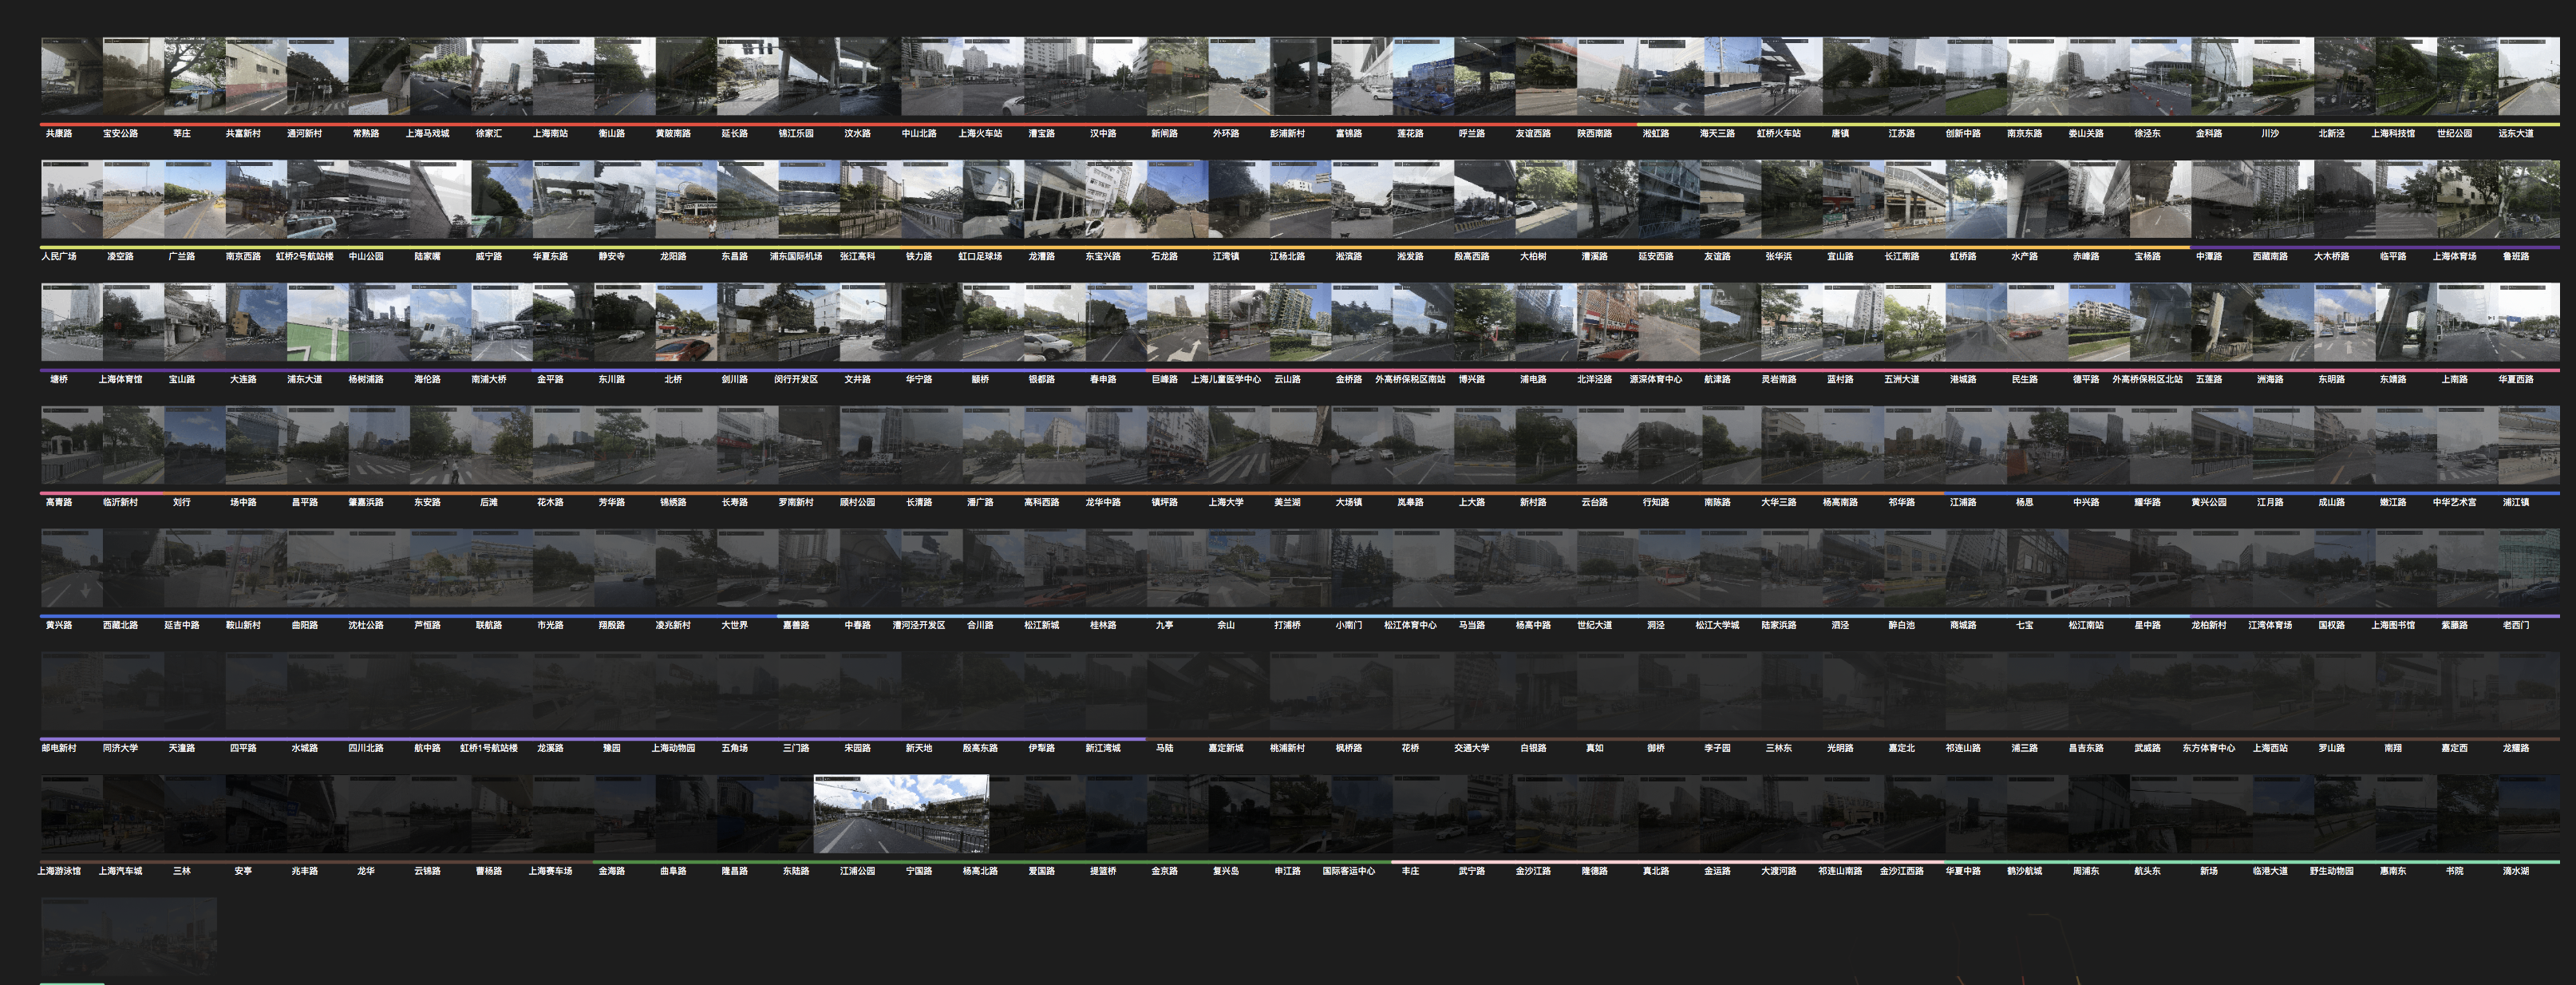
\includegraphics[width=0.5\textwidth]{img/EntranceFlow1}
	\caption{Entrance Flow}
	\label{fig:curve}
\end{figure}

The second half of Entrance Flow page presents a visualization for passenger volume. It consists of a metro map, an information board, and an interactive heat map. The heat map displays the intensity of passenger varies with time and metro stations. The horizontal axis of the heat map is metro station ordered by metro line and displayed in colorful aligning with metro lines. The vertical axis of the heat map is the exact time every 5 minutes. The interaction is designed to trigger highlights of the station in the metro map and displays of the information board by a click of the heat map. This design helps users not only have an overview of passenger volume at any time but also get details of metro station and passenger volume to do further analysis. 

\begin{figure}[t]
	\centering
	\includegraphics[width=0.5\textwidth]{img/EntranceFlow2}
	\caption{EntranceFlow - Heatmap}
	\label{fig:curve}
\end{figure}

\subsubsection{Exit Flow}
The exit flow is almost the same as the entrance flow. Differently, the data used here are the amount of passenger who exits the metro station. Another difference is the Exit Flow page only displays the heat map and the information board.



\section{Results}
\begin{enumerate}
\item \href{https://yutinghan.github.io/gradfinal/}{Weblink}
\item \href{https://www.youtube.com/watch?v=0AUQpKVXM7k&app=desktop}{Youtube video}
\end{enumerate}

\section{Discussion}
Nowadays, multiple metro visualization works are aiming at artistic presentation while some data developers have published some data works focusing on information expression. Our “One day of SHMetro” combines advantages of the above fields and presents Shanghai Metro’s flow in an aesthetic way with accurate messages.

\section{Conclusion}
Due to the limitations of data sources and our technical skills, our project remains improving in the coming future. 

First, we hope to call Shanghai Metro API to access real-time and completed data. If so, the visualization can be a scaled and comprehensive reflection of Shanghai transportation status. This could be implemented as metro data dashboard and could be used for urban research and analysis. 

Second, it will be meaningful to combine metro data visualization with other influence factors. For example, weathers or special events in the city can greatly influence passenger volume in metro stations. The user of our data dashboard can get a deeper understanding of passenger flow.

Third, to finalize the visualization project, we need to conduct marketing research on target users and get feedback. The opinions of users will help us better modify our design. 

All in all, “One day of SHMetro” bridges the gap between abstract metro flow with the concrete number and expresses urban analysis in an aesthetic way. 


\bibliographystyle{abbrv}
\bibliography{SHMetro}
\end{document}
